\documentclass{article}
\usepackage{enumitem}
\usepackage{graphicx}
\usepackage[letterpaper, margin=1in]{geometry}
\usepackage{times}
\usepackage{newtxtext}
\usepackage{multicol}  % Add this line for the multicol package
\usepackage{natbib}  
\usepackage{hyperref} 
\usepackage{float}
\usepackage{sectsty}
\usepackage{titlesec}


\titleformat{\section}[block]{\centering\bfseries}{\thesection.}{1em}{} % Centered section titles
\sectionfont{\fontsize{11}{15}\selectfont}
\subsectionfont{\fontsize{11}{14.4}\selectfont}  % Adjust the font size as needed
\subsubsectionfont{\fontsize{11}{13.2}\selectfont}  % Adjust the font size as needed


\begin{document}

\begin{titlepage}
    \centering
    
\includegraphics[width=0.6\textwidth]{images/logo.png}
    
    \vspace{2cm}

    {\fontsize{24pt}{28.8pt}\selectfont \fontfamily{ptm}\selectfont \textbf{Optimizing Home Energy Management: The Transformative Role of Progressive Web Apps (PWA) in Residential Electrical Measurements}}
    \vspace{1cm}
    
    {\Large Made by:}

    \vspace{1cm}

    {\fontsize{10pt}{28.8pt}\selectfont Gomez Leyva Jesus Armando}

    \vspace{0.5cm}
    {\fontsize{10pt}{28.8pt}\selectfont Luna Perez Cristian}

    \vspace{0.5cm}
    {\fontsize{10pt}{28.8pt}\selectfont Moreno Maya Marco Antonio}

    \vspace{0.5cm}
    {\fontsize{10pt}{28.8pt}\selectfont Labrada Galvez Antonio}
    
    \vspace{2cm}
    
    {\large January 17th, 2024}
    
\end{titlepage}

\begin{multicols}{2}  % Start two-column layout

\section*{EXECUTIVE SUMMARY}
This document explores the integration of Progressive Web Apps (PWA) into residential electrical measurement applications, offering an efficient and accessible solution to empower users in monitoring and managing their energy consumption.

\section*{INTRODUCTION}
The increasing prevalence of connected devices in modern homes has underscored the critical need for advanced solutions in residential electrical measurement. As we delve into this exploration, we will address the challenges posed by conventional applications in terms of accessibility, updates, and performance (Chapter 2). In response to these challenges, we propose the integration of Progressive Web Apps (PWAs) as a transformative solution, unlocking efficient and accessible avenues for users to monitor and manage their energy consumption (Chapter 4).

This document will unfold in a structured manner, commencing with an overview of the current landscape in residential electrical measurement and the associated challenges (Chapter 2). Subsequently, we will delve into the capabilities of PWAs and how they can revolutionize the user experience, emphasizing features such as offline accessibility, automatic updates, and cross-device compatibility (Chapter 3). To demonstrate the practical implications of our proposal, we will present real-world use cases showcasing the versatility of PWAs in enhancing residential electrical measurements (Chapter 5).

Furthermore, we will explore the advantages and benefits of adopting PWAs, including improved accessibility from mobile devices, seamless updates, offline access to consumption data, enhanced performance, and increased user engagement (Chapter 6). Security and privacy concerns, pivotal in the implementation of PWAs, will be thoroughly addressed, emphasizing encryption, authentication mechanisms, secure storage, and adherence to legal compliance (Chapter 7).

In conclusion, we will summarize the transformative potential of PWAs in residential electrical measurement, emphasizing the holistic solution they offer to the limitations of traditional applications (Chapter 8). Finally, we will provide practical recommendations for utility providers and developers to adopt PWAs, ensuring an enhanced experience for end-users (Chapter 9).

\section*{PROBLEM DESCRIPTION}
Conventional home electrical measurement applications are often limited in terms of accessibility, automatic updates, and performance. These challenges impact users' ability to understand and efficiently manage their energy consumption.

\section*{PWA IN RESIDENTIAL ELECTRICAL MEASURUMENT}

Optimizing Residential Electrical Measurement with Progressive Web Apps (PWA)
In this comprehensive exploration, we delve into how Progressive Web Apps (PWAs) can effectively overcome existing limitations in residential electrical measurement applications. By offering swift and convenient access from any device, even in environments with variable connectivity, PWAs prove to be a transformative solution.
\begin{itemize}
    \item \textbf{Offline Accessibility:} Progressive Web Apps revolutionize the accessibility of residential electrical measurement data, ensuring users can access crucial information even without a continuous internet connection. This feature enhances usability in various scenarios, providing uninterrupted access to vital data when users need it most.
    \item \textbf{Automatic Updates:} Seamless updates are a hallmark of PWAs, allowing applications to adapt promptly to changes in rates, regulations, or the introduction of additional features. Users can be confident they always have the most up-to-date information at their fingertips, enhancing the reliability and relevance of the application.
    \item \textbf{Cross-Device Compatibility:} With PWA implementation, users gain the flexibility to monitor their energy consumption seamlessly across a diverse range of devices. Whether using smartphones, tablets, or desktop computers, the cross-device compatibility of PWAs significantly enhances accessibility and convenience. Users can effortlessly transition between devices while maintaining a consistent and user-friendly experience.
\end{itemize}
By incorporating these key features, our PWA solution for residential electrical measurement not only addresses current limitations but also sets the stage for a more accessible, reliable, and user-centric experience. This innovative approach ensures that users can efficiently manage their energy consumption regardless of their internet connectivity or the device they choose to use.

\section*{PRACTICAL USE CASES}
Examples illustrating how PWAs can be used in everyday situations, enhancing the experience of residential electrical measurements:

\begin{enumerate}
    \item \textbf{Remote Monitoring:} Utilize the PWA to remotely monitor real-time energy consumption from a mobile device, providing users with instant access to their home's electrical data.
    
    \item \textbf{Alerts for Consumption Peaks:} Implement an alert system within the PWA to notify users when their energy consumption exceeds predefined thresholds. This feature empowers users to take immediate actions in response to unexpected spikes in usage.
    
    \item \textbf{Detailed Energy Usage Analysis:} Enable users to conduct in-depth analyses of their energy usage patterns through the PWA. Utilize interactive graphs and charts to present historical data, helping users make informed decisions about energy-saving strategies.
\end{enumerate}

\section*{ADVANTAGES AND BENEFITS}
\begin{itemize}
    \item \textbf{Accessibility from Mobile Devices:} Users enjoy seamless access to the residential electrical measurement application from a diverse array of mobile devices, providing unparalleled convenience and flexibility. This ensures that users can effortlessly manage and monitor their energy consumption on the go.
    
    \begin{figure}[H]
        \centering
        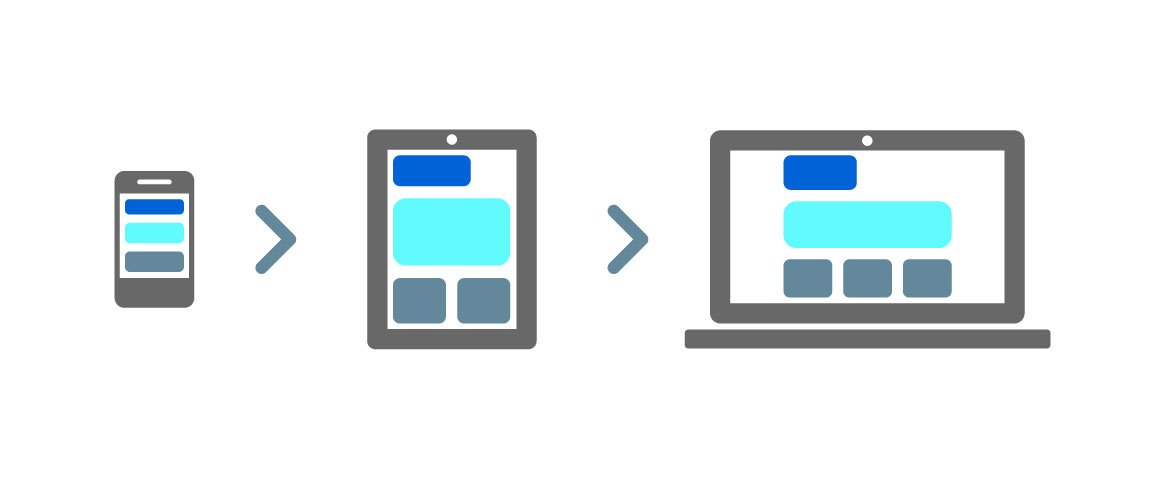
\includegraphics[width=0.8\linewidth]{images/mobile-first.jpg}  % Adjust the width as needed
        \caption{PWA allows you to use your application across all devices.}
    \end{figure}

    \item \textbf{Automatic Updates:} Progressive Web Apps (PWAs) facilitate automatic updates, eliminating the need for manual intervention. This ensures that the application consistently reflects the latest changes in rates and features, keeping users informed with up-to-date information without any hassle.
    
    \item \textbf{Offline Access to Consumption Data:} PWAs empower users with the ability to access their energy consumption data even in offline mode. This feature guarantees uninterrupted insights into usage patterns, allowing users to stay informed about their electricity consumption regardless of internet connectivity.
    
    \item \textbf{Improved Performance:} Leveraging PWA's intelligent resource caching capabilities, the application exhibits enhanced performance, particularly in environments with variable connectivity. This not only ensures a smooth user experience but also optimizes performance even in challenging network conditions.
    
    \item \textbf{Enhanced User Engagement:} PWAs, renowned for their accessibility and user-friendly design, contribute to heightened user engagement. This fosters a deeper understanding of energy consumption patterns, encouraging users to make informed decisions about their electricity usage. The intuitive nature of the application promotes a more interactive and satisfying user experience.
\end{itemize}
Incorporating these advantages, our PWA solution not only ensures the efficient management of residential energy consumption but also provides users with a robust, reliable, and engaging platform tailored to their convenience and evolving needs.


% Continue the rest of your document...


\section*{SECURITY AND PRIVACY}
Addressing concerns about data security and privacy is paramount in the implementation of Progressive Web Apps (PWAs) for residential electrical measurement. The following considerations demonstrate how PWAs can implement robust security measures and respect user privacy:

\begin{itemize}
    \item \textbf{Data Encryption:} Ensure that all communication between the PWA and the backend servers is encrypted using secure protocols such as HTTPS. This prevents unauthorized access to sensitive user data during transmission.

    \item \textbf{Authentication Mechanisms:} Implement strong user authentication mechanisms to verify the identity of users accessing the PWA. This can include multi-factor authentication for an additional layer of security.

    \item \textbf{Secure Storage:} Utilize secure storage mechanisms for storing sensitive data on the user's device. This helps protect user information even in the event of device loss or theft.

    \item \textbf{Privacy by Design:} Design the PWA with privacy in mind, following the principles of privacy by design. Minimize data collection to only what is necessary for the application's functionality, and obtain user consent for data processing.

    \item \textbf{User Consent and Transparency:} Clearly communicate to users about the types of data collected, how it will be used, and obtain explicit consent. Users should have control over their data and be informed about any changes in privacy policies.

    \item \textbf{Regular Security Audits:} Conduct regular security audits to identify and address potential vulnerabilities. Keep the PWA and associated systems up-to-date with the latest security patches.

    \item \textbf{Legal Compliance:} Ensure compliance with relevant data protection regulations and laws. This may include GDPR, CCPA, or other regional privacy regulations depending on the user base.
    
    \citep{Security}
\end{itemize}

\section*{CASE STUDY}

\section*{1. Twitter Lite}

Twitter successfully implemented a Progressive Web App (PWA) version, known as Twitter Lite, which has significantly enhanced user accessibility. The streamlined PWA not only offers a faster and more reliable experience but also reduces data usage, contributing to overall energy efficiency for users.
\citep*{BestPWAExamples}
\section*{2. Flipkart}

The e-commerce giant Flipkart adopted a PWA strategy, resulting in remarkable success. The PWA version of Flipkart provides users with a smooth shopping experience, even in low-connectivity environments. The optimized performance not only boosts user engagement but also contributes to energy savings by reducing the strain on data networks.
\citep*{PWAcaring}
\section*{3. Starbucks}

Starbucks, a global leader in the food and beverage industry, successfully implemented a PWA to enhance the customer experience. The Starbucks PWA allows users to order ahead, customize their drinks, and find nearby stores seamlessly. This not only improves efficiency for users but also contributes to energy savings by reducing the need for in-store wait times.
\citep{StarbucksPWA}


\section*{CONCLUSIONS}
In conclusion, the integration of Progressive Web Apps (PWAs) into residential electrical measurement applications represents a transformative step towards enhancing user experience and promoting efficient energy management. By addressing the limitations of traditional applications, PWAs offer quick and accessible access to consumption data, automatic updates, and offline functionality.



The advantages and benefits of implementing PWAs in this context, such as improved accessibility from mobile devices and real-time updates reflecting changes in energy rates, contribute to empowering users in their efforts to monitor and manage energy consumption effectively. Practical use cases demonstrate the versatility of PWAs, enabling remote monitoring, timely alerts for consumption peaks, and detailed analysis of energy usage within the home.



Security and privacy considerations have been thoroughly addressed, assuring users that the implementation of PWAs in residential electrical measurement applications prioritizes robust security measures and respects user privacy.



In summary, the adoption of PWAs offers a holistic solution to the challenges faced by conventional applications, enabling users to make informed decisions, enhancing energy efficiency, and ultimately transforming the way residential energy consumption is monitored and managed.

   
\bibliographystyle{plainnat} % Choose a bibliography style
    \bibliography{references.bib} 
\end{multicols}  % End two-column layout
\end{document}